%\chapter{Effect of Xenon on the overall thermal conductivity of \protect\NoCaseChange{U--{10}Mo}}
\chapter{Estimation of Effective Thermal Conductivity in \protect\NoCaseChange{U-10Mo} fuels with distributed xenon gas bubbles}
\textit{This chapter was published as an article in the \textup{Journal of Nuclear Materials}. The authors of that article are A. Rafi M. Iasir and Karl D. Hammond of the University of Missouri and Nickie J. Peters of the University of Missouri Research Reactor Center.}

\section{Introduction}\label{sec:introduction}
The Reduced Enrichment for Research and Test Reactors (RERTR)~\cite{snelgrove1997development} program was initiated in the USA in the late 1970s to develop new nuclear fission fuels to replace high-enrichment uranium (HEU)\@. The development of low-enrichment uranium (LEU) fuels for high-performance reactors is an important nonproliferation initiative~\cite{snelgrove1997development}. One of the main requirements of LEU fuels is increased uranium density, such as that found in metallic uranium, to offset the decrease in \textsuperscript{235}U enrichment. Metallic uranium is thought to have sufficient density, but the orthorhombic crystal structure of \textalpha-uranium
and the anisotropic fuel swelling that results make it unattractive as a fuel.
Uranium alloys that retain the high-temperature \textgamma-phase, which is body-centered cubic, are more suitable for reactor fuel due to their more isotropic radiation-induced swelling behavior compared with  \textalpha-uranium~\cite{kittel1993history}.

Various uranium alloys have been tested as alternative metallic fuels under reactor operating conditions, including U$_6$Fe and U$_6$Mn~\cite{meyer2000irradiation,hofman1987irradiation}.
%The U-Mo alloy has been identified as a high-performance fuel due to its high uranium density and low neutron capture cross-section~\cite{ewh2010microstructural,smirnova2013ternary,rest2009analysis,landa2013density}.
Elements such as molybdenum (Mo), niobium (Nb), titanium (Ti), and zirconium (Zr) have also been tried as alloying elements because of their solubility in \textgamma-uranium~\cite{donze1959stabilisation,giraud1973formation,lopes2013mechanical}. Molybdenum stabilizes uranium's \textgamma-phase at concentrations near the eutectoid point, lowering the phase transition temperature from 776~\textdegree C for pure uranium (corresponding to the \textbeta--\textgamma\ allotropic point) to the eutectoid point of 555~\textdegree C for 11.1~percent molybdenum in \textgamma-uranium by weight~\cite{ASM-Alloy-Mo,Berche2011}. To take advantage of this, uranium alloyed with 10 wt$\%$ molybdenum (U-10Mo) is currently being developed as a potential high-density LEU fuel for high-performance research reactors.

The two major fuel types are U--Mo/Al dispersion fuels (U--Mo grains dispersed in an aluminum matrix) and U--Mo monolithic fuels~\cite{keiser2012effects}. Dispersion fuels show poor irradiation performance due to fuel--matrix interaction, which causes break-away swelling behavior at intermediate burnup~\cite{hofman2004post,van2008transmission, leenaers2004post}. In monolithic fuels, a zirconium foil is used as a diffusion barrier between the fuel and the cladding (aluminum) to prevent diffusion of molybdenum into the cladding~\cite{jue2014microstructural}.

Thermal conductivity is an important property of any nuclear fuel, since most of the important physical properties are temperature-dependent. In the case of high-performance reactors, fuels must undergo high fission density at relatively low temperatures. For this reason, research reactor fuels are designed for efficient heat rejection. During test operations, Burkes and coworkers~\cite{burkes2015thermal} observed that the thermal conductivity in monolithic fuels decreased significantly with increased burnup. For a fission density of $3.30\times10^{21}$~fissions/cm$^3$ at 200~\textdegree C, thermal conductivity decreased by approximately 30\%; at $4.53\times10^{21}$~fissions/cm$^{3}$, conductivity decreased by 45\%~\cite{burkes2015thermal}.

Fission also creates a variety of fission products, which result in gas
bubbles, metallic precipitates, and solutes in the fuel
matrix~\cite{rondinella2010high}. These fission products, in addition to
radiation damage in reactor environments, result in complex microstructural
evolution that restructures the nuclear fuel over time. Fission gas bubbles are
particularly problematic, as they cause changes in thermal conductivity and
swelling of the fuel. In addition, \textsuperscript{135}Xe is a potent neutron
absorber. {Solid fission products (e.g., Sr, Y, Zr, La, Ce,
and Nd)\ are also constantly being produced; these elements can form
intermetallic alloys, which can increase the volume of the fuel and reduce the
thermal diffusivity~\cite{ishimoto1994effects, kang2007thermal}. These solid
fission products also play an important role in the thermal stability of
fission gas bubbles~\cite{gan2015thermal}.} 

For every four fission events, an average of one inert gas atom (xenon or krypton) is produced. The dominant gaseous species is xenon, accounting for almost $85\%$ of fission gas~\cite{blades1956ratio,petruska1955absolute}. Xenon atoms in U--Mo alloy fuels have a strong tendency to precipitate into small bubbles due to their low solubility. The formation and growth of gas bubbles inside irradiated nuclear fuels has technical importance, as bubbles influence the microstructure of the material~\cite{kim2011fission}. Recent TEM and SEM images show that fission bubbles in U-10Mo distribute themselves in both inter-granular and intra-granular formations~\cite{miller2015transmission,miller2012advantages, gan2012tem, gan2010transmission}. High-fission-density fuels show randomly-distributed, micrometer-sized fission gas bubbles distributed throughout the grains~\cite{gan2012tem}. Inter-granular bubble density increases with burnup. 

Inside the micrometer-sized grains, fission gas forms superlattices~\cite{miller2015transmission,miller2012advantages, gan2012tem},
similar to those seen in ion-irradiated materials~\cite{johnson1980gas, johnson1980hydrogen, evans1983void, mazey1986bubble, evans1986solid, johnson1991image, johnson1995gas, lawson1998temperature, ghoniem2001theory,johnson2006helium}. Typical bubble sizes are 2--6~nm in diameter, and the distance between the bubbles is typically in the 4--12 nm range. The superlattice usually has the same crystal structure as the host material, but an exception exists: the superlattice in U-10Mo shows a face-centered cubic structure in a body-centered cubic matrix. An ion-irradiated bubble superlattice has a lattice parameter of tens of nanometers~\cite{miller2015transmission}; that of fission gas bubbles is
typically similar~\cite{Gan2015}.
The superlattice forms in ion-irradiated materials between approximately
$0.15T_m$ and $0.35T_m$~\cite{lawson1998temperature}, which is within the
typical anticipated operating range of \mbox{U--Mo} fuels, and the superlattice
in \mbox{U-10Mo} can survive temperatures up to approximately
850~\textdegree C~\cite{Gan2015}.

The thermal conductivity of a monolithic \mbox{U--Mo} fuel plate is at a maximum prior to irradiation~\cite{burkes2015thermal}.
Inclusions and porosity change the thermal and the electrical conductivity of many materials~\cite{bakker1997using}. 
Solid fission products usually have minimal impact on overall thermal conductivity, as their conductivities are similar to the conductivity of the fuel. Gases, on the other hand, have much lower thermal conductivity than
the matrix, and typically have much lower densities and heat capacities as well. Various models, both empirical and theoretical, have been proposed to describe the changes in conductivity due to gas bubbles. Maxwell~\cite{maxwell1881treatise} was among the first to derive an expression for the effective thermal conductivity of heterogenic media; his model assumed a uniform distribution of spherical particles in a matrix. A few other empirical models also exist~\cite{macewan1967effect,goldsmith1973measurements,devries1989experimental}; unfortunately, the large diversity of pore shape, pore size, and type of included material inside nuclear fuel make it impossible to describe heat transfer with a single equation. Several theoretical models have been proposed to describe the influence of porosity and inclusions on the thermal conductivity~\cite{maxwell1881treatise,loeb1954thermal, cunningham1981heat, tzou1991effect, bauer1993general}. These theoretical models usually assume pores with regular geometric shapes and that the pore arrangement is sufficiently dilute so as to neglect interaction between inclusions.

The microstructure of irradiated nuclear fuels is very complicated due to the lack of consistency between bubbles. The intra-granular gas bubbles are two or three orders of magnitude smaller than the inter-granular gas bubbles~\cite{hu2015assessment}. The shapes of the bubbles are also highly variable: the intra-granular gas bubbles are approximately spherical, whereas inter-granular gas bubbles do not have consistent shapes. In this work, we assess contributions to the thermal conductivity of \mbox{U-10Mo} from both inter- and intra-granular gas bubbles. The impact of xenon bubble pressure on the overall thermal conductivity is also estimated.
{Because fission gas is typically a mixture of krypton and
xenon, rather than pure xenon, we include two comparisons with a krypton--xenon
mixture.}
At the end, we present a study of the influence of different bubble arrangements on the overall thermal conductivity.

 

\section{Methods} \label{sec:Methodology}
A finite element model was used to solve the steady-state heat conduction equation in the presence of various microstructures. Two types of microstructures containing xenon gas bubbles were used: a xenon bubble superlattice structure representing intra-granular bubbles, and a grain boundary structure representing inter-granular bubbles. Figure~\ref{gbs} shows an example of an intra-granular bubble distribution, while Figure~\ref{fig_Xe_SEM} shows the inter-granular bubble distribution.
In the intra-granular bubble case, xenon gas bubbles were placed in a variety
of spatial configurations, including configurations consistent with a gas bubble superlattice.
\begin{figure}%[H]
    \centering
	  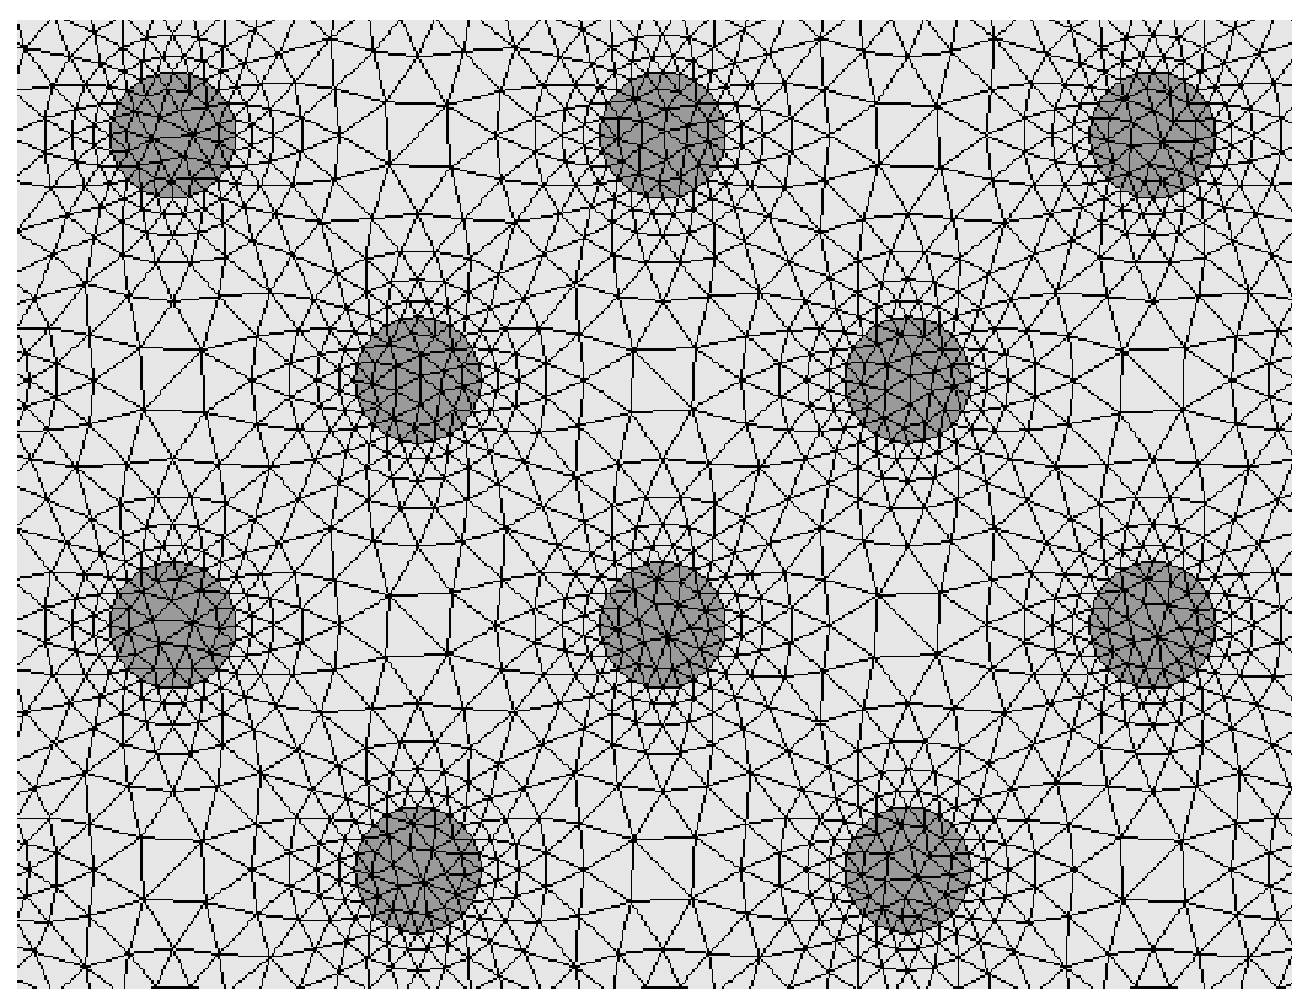
\includegraphics[width=3.25in]{meshed_figure_GBS_gray}
    \\
	 
\includegraphics[width=3.25in]{figure_GBS_fcc_2_gray}
	\caption[(a)~Discretized domain of intra-granular xenon bubbles inside a U-10Mo matrix; (b)~Example two-dimensional bubble distribution 
used for intra-granular xenon gas, consisting of bubbles with 3.1, 3.6, 3.75,
        and 4.0~nm diameters, consistent with the work of Miller and
        coworkers]{(a)~Discretized domain of intra-granular xenon bubbles inside a U-10Mo matrix; (b)~Example two-dimensional bubble distribution 
used for intra-granular xenon gas, consisting of bubbles with 3.1, 3.6, 3.75,
        and 4.0~nm diameters, consistent with the work of Miller and
        coworkers~\cite{miller2015transmission}. The lattice parameter for the
        gas bubble superlattice is 12.0~nm.}
	\label{gbs}
\end{figure}
All simulations were performed in a two-dimensional domain. The gas bubble supperlattice structure was created based on data from Miller \etal~\cite{miller2015transmission}. According to Miller \etal~\cite{miller2015transmission}, the bubble size inside the grain boundary superlattice structure is normally distributed. Based on their experimental values, we chose four bubble diameters to create our simulation. Because the superlattice in U-10Mo is FCC, the two-dimensional structure of bubbles was created based on the FCC structure with a 12~nm lattice parameter, which was also taken from Miller \etal~\cite{miller2015transmission}. The bubble sizes were randomly sampled from this distribution using the discrete values of 3.1, 3.6, 3.75, and 4.0~nm in diameter. The square domain's dimensions were 80~nm${}\times{}$80~nm, which results in 85 bubbles with a lattice constant of 12~nm. Triangular elements were used to create the mesh using the Trelis Pro software package~\cite{trelis}.

In the inter-granular bubble case, the grain boundary structure of U-10Mo was created based on images from Miller \etal~\cite{miller2012advantages}. Their SEM (scanning electron micrograph) of a focused ion beam (FIB) cross-section showed fission gas bubbles populating the grain boundaries, as shown in Figure~\ref{fig_Xe_SEM}. This domain was also discretized with triangular elements. The top and bottom boundaries of the domain of the FEM domain were assumed to be adiabatic. The left and right boundaries have fixed-temperature boundary conditions applied. This temperature difference drives the heat flow. 


\begin{figure}%[t]
\centering
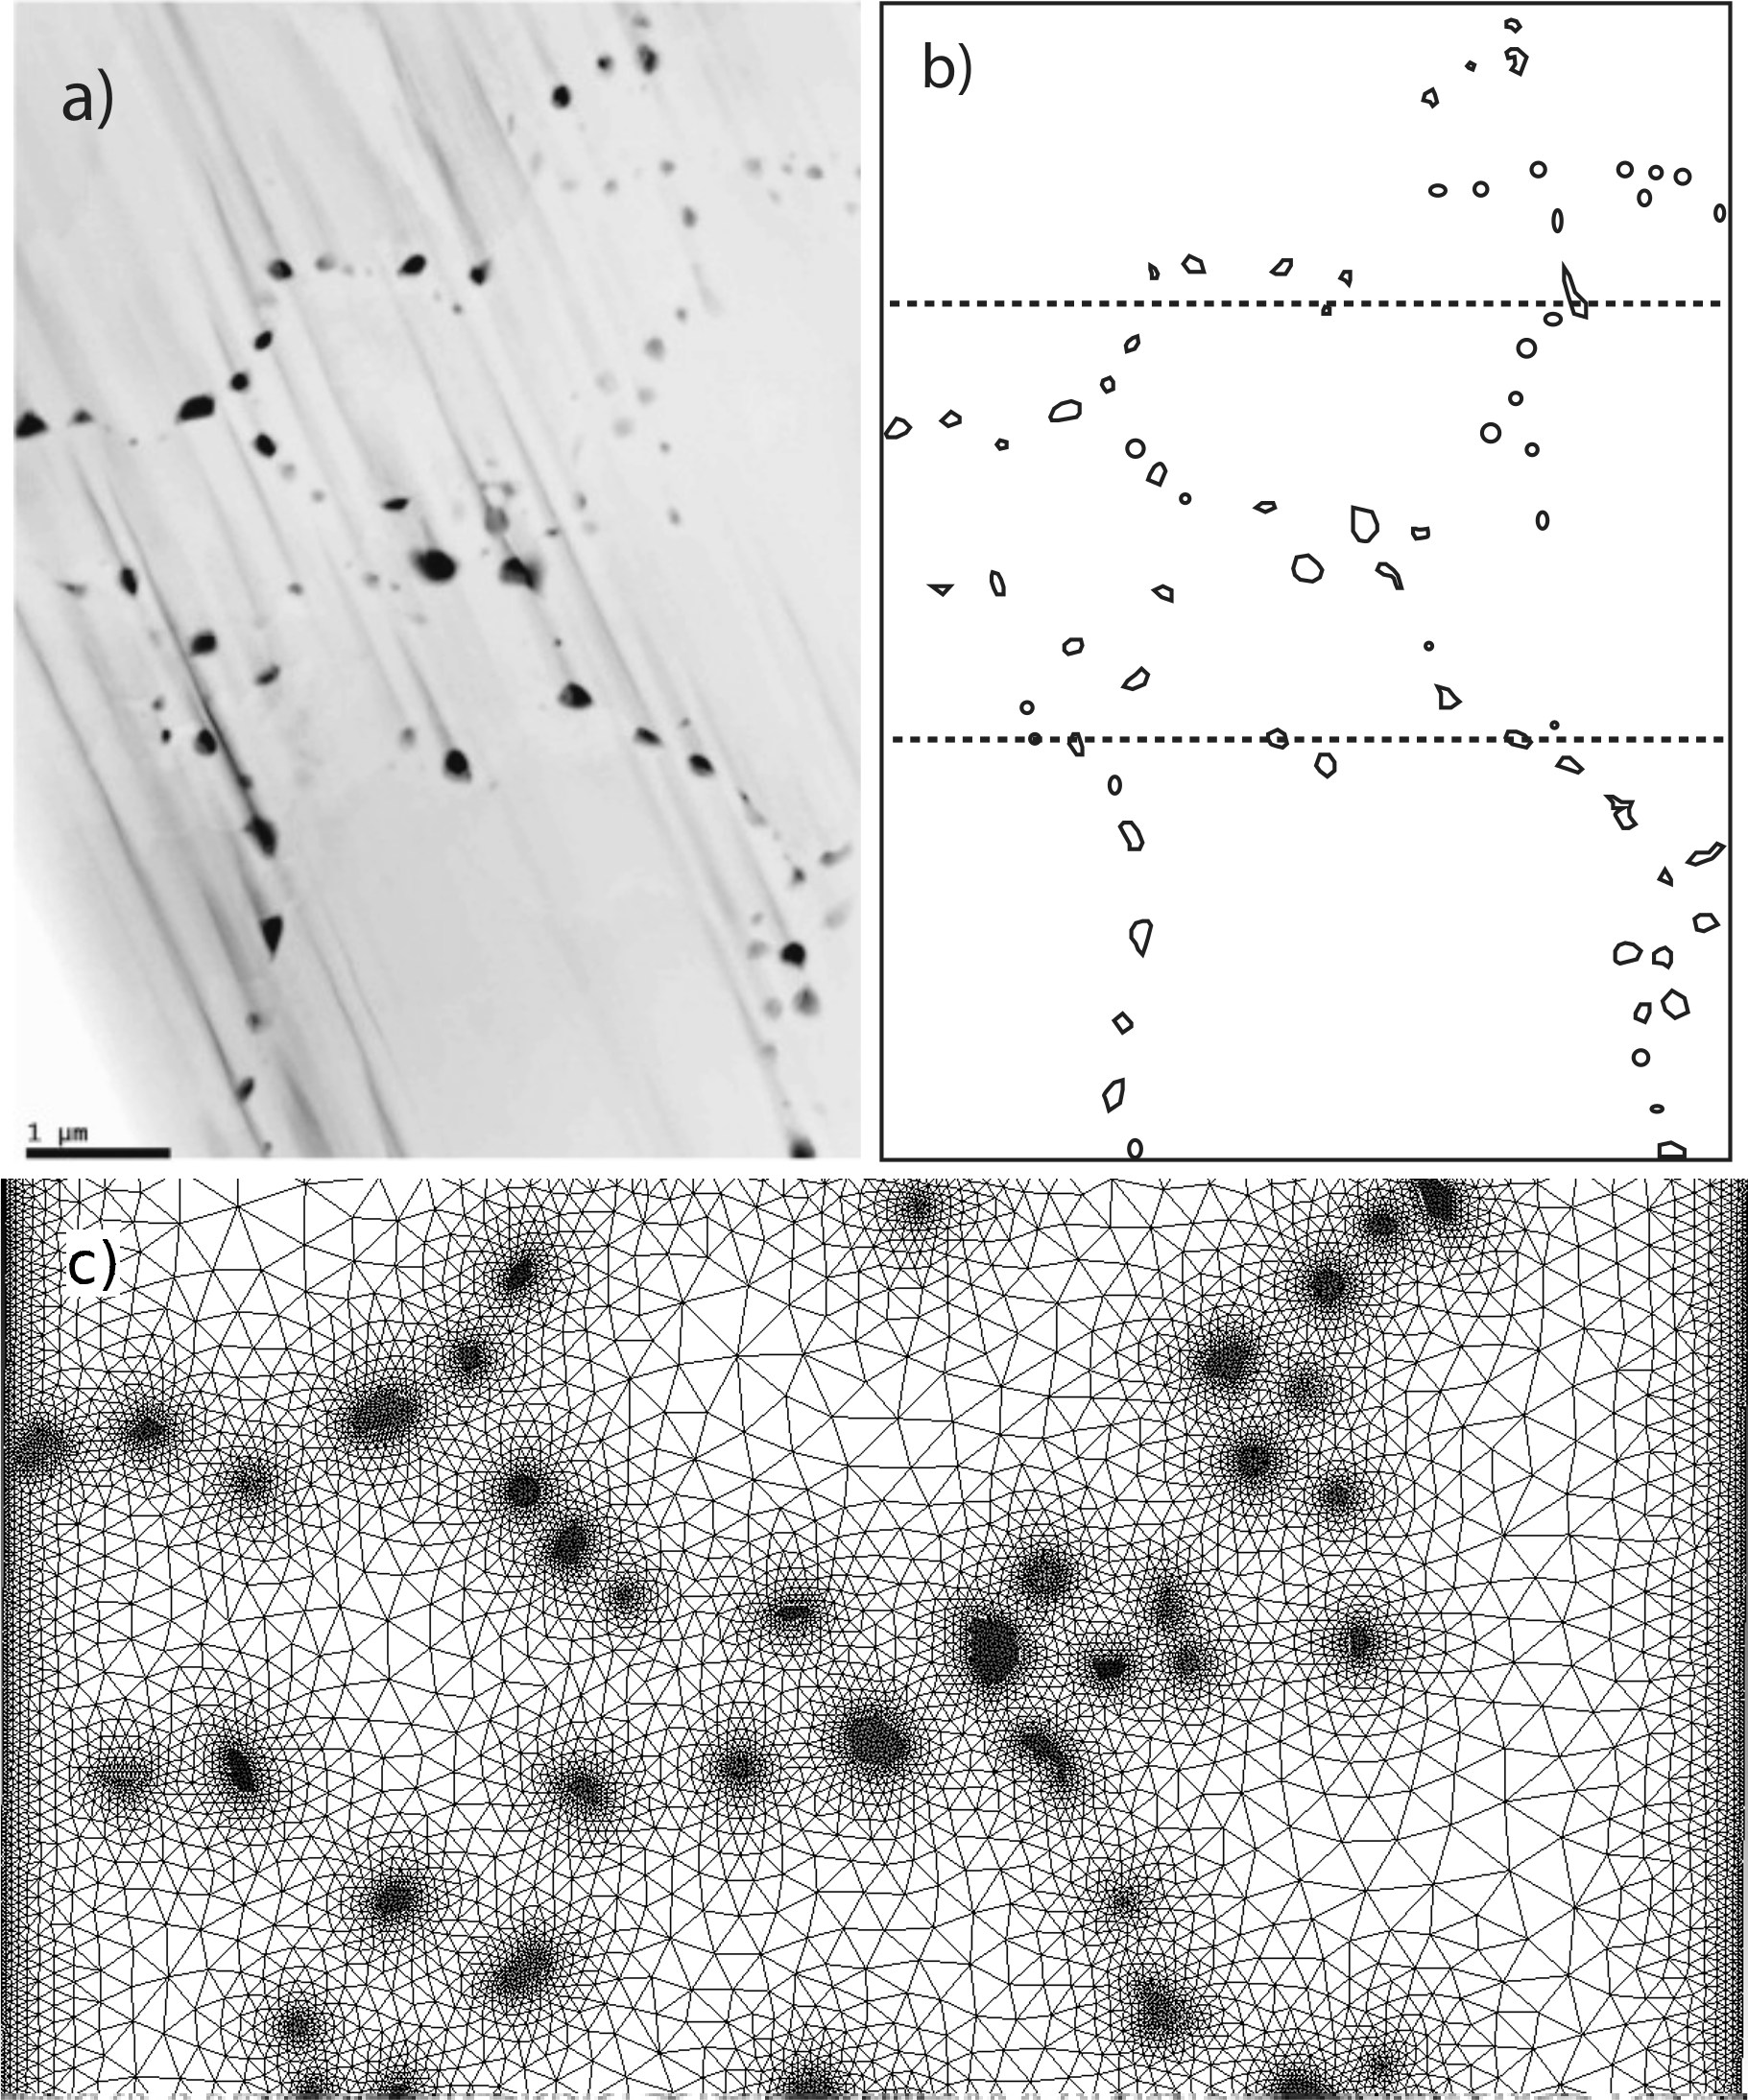
\includegraphics[width=90mm]{grain_boundary_U-10Mo_white_BG}
\caption[(a) SEM image of the fission gas bubbles along the grain boundaries from Miller used for FEM calculations (b) Geometry created based on the grain boundary fission gas image in (a) (c) FEM mesh with grain boundary fission gas of the region between the dotted line in  (b).]{(a) SEM image of the fission gas bubbles along the grain boundaries from Miller \etal~\cite{miller2012advantages} used for FEM calculations (b) Geometry created based on the grain boundary fission gas image in (a) (c) FEM mesh with grain boundary fission gas of the region between the dotted line in  (b). }
\label{fig_Xe_SEM}
\end{figure}
\begin{figure}
\centering
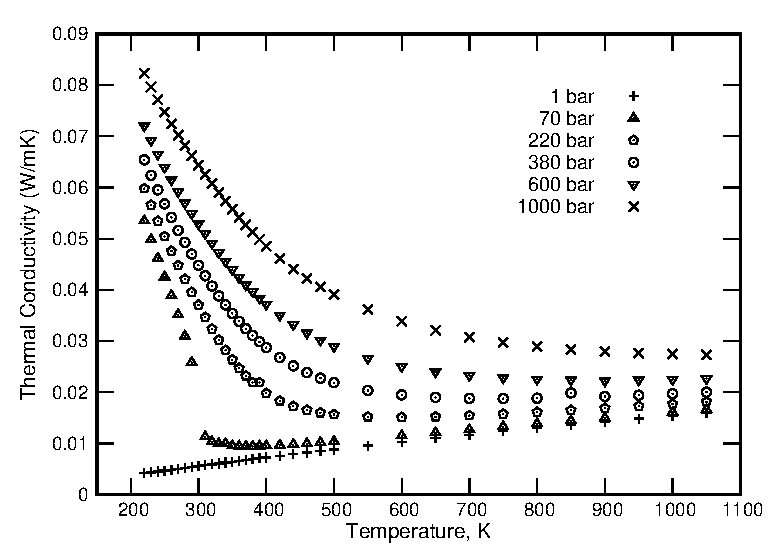
\includegraphics[width=110mm]{Xe_K_eps_rotate}
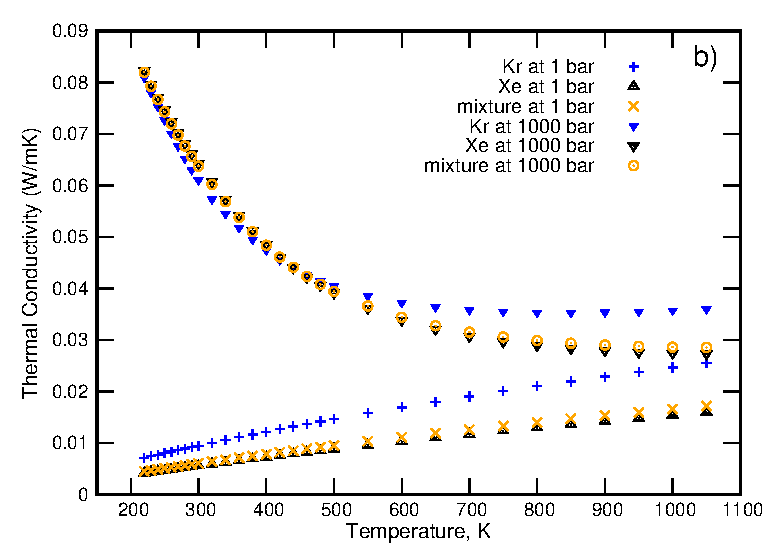
\includegraphics[width=110mm]{krypton_xenon_compare}
\caption[(a) Thermal conductivity of xenon as a function of pressure and
temperature based on the measurements of Rabinovich et
al.]{(a) Thermal conductivity of xenon as a function of pressure and
temperature based on the measurements of Rabinovich et
al.~\cite{rabinovich1987thermophysical}.  Note that the critical point of xenon
is 289.733~K and 58.42~bar; this is why there is such a drastic change in
conductivity at low temperature between the 1~bar and 70~bar isobars.
{(b) Comparison between the thermal conductivities of pure
krypton and pure xenon (both at 1~bar and at 1000~bar) with a mixture of
15\% krypton and 85\% xenon at both 1~bar and 1000~bar. This composition is
representative of fission gas.}}
\label{fig_Xe_pressure}
\end{figure}

The thermal conductivity of \mbox{U-10Mo} was estimated from a linear fit of thermal conductivity as a function of temperature between 298~K and 1073~K from Kaufmann~\cite{kaufmann1962nuclear}. Burkes \etal~\cite{burkes2010thermo} also provided a linear fit of the \mbox{U-10Mo} thermal conductivity as a function of temperature up to 873~K; their results were in good agreement with Kaufmann's~\cite{kaufmann1962nuclear}.
{Xenon conductivity is drawn from the data of Rabinovich \etal~\cite{rabinovich1987thermophysical};}
the thermal conductivity of xenon depends on both temperature and pressure,
as shown in Figure~\ref{fig_Xe_pressure}. The pressure inside a bubble depends on the radius of the bubble, the surface tension, the magnitude of the Burgers vector, and the shear modulus of the host material~\cite{greenwood1959role,trinkaus1983energetics}. According to Xiao \etal~\cite{xiao2015atomistic}, the pressure inside a xenon bubble can be as high as 120~kbar. Such high pressures suggest the possibility of forming solid xenon bubbles inside the fuel~\cite{thomas1991condensed,ross1980condensed,zheng2014thermodynamics}. Unfortunately, thermal conductivity data for xenon above 1000~bar are not available, so we chose two limiting sets of thermal conductivity data: 1~bar and 1000~bar. For each set of data, a polynomial fit (fifth order) was used to interpolate the conductivity over the temperature range.
{Fission gas is typically a mixture of krypton and xenon, so
we ran simulations in which the bubbles were filled with 15\% krypton,
85\% xenon (molar basis), with conductivity data for krypton from Rabinovich \etal~\cite{rabinovich1987thermophysical}. The mixture's thermal conductivity was calculated using Wilke's mixing rule~\cite{wilke1950viscosity}, which uses the full first-order Chapman--Enskog relation along with Eucken's relation for the thermal conductivities~\cite{vincenti1965introduction, alkandry2013comparison}. Using Wilke's approach, the mixture's thermal conductivity is given by
\begin{equation}
  K = \sum_i \frac{x_iK_i}{\sum_j x_j \phi_{ij}},
  \label{eq:K-mixture}
\end{equation}
where $x_i$ is the mole fraction and $K_i$ is the conductivity of the pure
component. The coefficients $\phi_{ij}$ can be calculated by the following
relation~\cite{alkandry2013comparison}:
\begin{equation}
  \phi_{ij} = \frac{\left[1+\left(\dfrac{\mu_i}{\mu_j}\right)^{\!\!1/2}\left(\dfrac{M_j}{M_i}\right)^{\!\!1/4}\right]^2}{\left[
    8\left(1+\dfrac{M_i}{M_j}\right)
  \right]^{1/2}},
\end{equation}
where $M_i$ is the molar mass of the species and $\mu_i$ is the viscosity.
}
\nomenclature{$K$}{thermal conductivity}
\nomenclature{$x_i$}{mole fraction}
\nomenclature{$M_i$}{molar mass}

\subsection{Effective Thermal Conductivity Calculation}
\label{subsec:Keffcalc}
The temperature in a composite material in the absence of heat sources is described by the heat equation:
\begin{equation}
\nabla \cdot \left(K\nabla T \right)=0,
\label{eq:Tdiff}
\end{equation}
where $K(x,y)=\chi_1(x,y)K_1 + \chi_2(x,y)K_2$ is the thermal conductivity tensor, $T$ is the temperature, $K_i\ { }(i=1$ for the matrix and 2 for the bubble) is the thermal conductivity tensor, and $\chi_i(x,y)$ is the indicator function of phase $i$. The local heat flux can be calculated using the equation
\begin{equation}
\label{eq:localflux}
q''(x,y) = -K(x,y) \cdot \nabla T(x,y),
\end{equation}
where $q''(x,y)$ is the local heat flux vector and $\nabla T(x,y)$ is the local temperature gradient. The local temperature and heat flux are calculated by solving Equations~\eqref{eq:Tdiff} and \eqref{eq:localflux}. The components of the effective thermal conductivity tensors are calculated via 
\begin{equation}
\label{eq:Keffcalc}
K_{\text{eff}}^x = -q_x''\left<\frac{\partial x}{\partial T}\right>.
\end{equation}
Where $q''_x$ is the mean heat flux in the $x$-direction, and $\left<\frac{\partial x}{\partial T}\right>$ is the average inverse temperature gradient in the $x$-direction. The MOOSE Framework~\cite{gaston2009moose} was used to solve Equation~\eqref{eq:Tdiff} with Dirichlet boundary conditions at $x=0$ and $x=L$ and Neumann (adiabatic) boundary conditions at $y=0$ and $y=L$. The effective thermal conductivity was calculated using Equation~\eqref{eq:Keffcalc}.



\section{\label{sec:results}Results and Discussion}
%The presence of xenon bubbles which have relatively low thermal conductivity in U-10Mo fuel effectively reduces the heat flow area and thus impacts the rate of overall heat transfer. Xenon bubbles have a broad range of diameters~\cite{miller2015transmission}; the size of the bubbles depends on the fission density and irradiation time. Due to significant size differences between intra- and inter-granular gas bubbles, the calculation of effective thermal conductivity was divided into two steps. In the first step, the thermal conductivity of a single crystal with nanometer-sized intra-granular gas bubbles was calculated. In the second step, the overall thermal conductivity of a polycrystalline material with intra- and inter-granular gas bubbles was calculated. 

\subsection{Effect of Xenon Gas Bubbles on the Thermal Conductivity} 
\label{subsec:xenonbubble}
We examined two broad categories of bubbles: inter-granular bubbles (\ie,
bubbles that collect at grain boundaries) and intra-granular bubbles.
The intra-granular case is intended to represent the effect of a gas bubble
superlattice (GBS) on the conductivity. We will discuss each case in turn.

\subsubsection{Intra-Granular Bubbles}
\begin{figure}%[H]
\centering
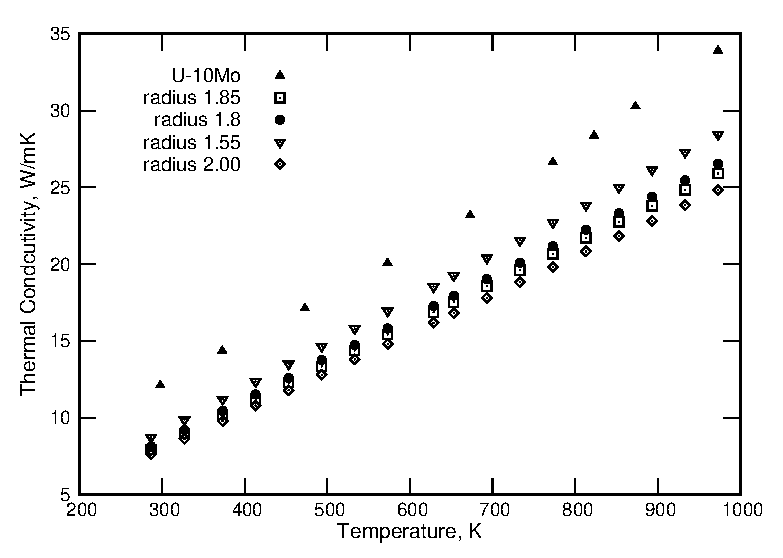
\includegraphics[width=110mm]{result_eps_rotate_bold}
\caption[Comparison between the thermal conductivity of \mbox{U-10Mo}
  (from Kaufmann) to the effective thermal
  conductivity of \mbox{U-10Mo} with intra-granular xenon bubbles of different
  diameters as arranged in Figure~\ref{gbs}b.]{Comparison between the thermal conductivity of \mbox{U-10Mo}
  (from Kaufmann~\cite{kaufmann1962nuclear}) to the effective thermal
  conductivity of \mbox{U-10Mo} with intra-granular xenon bubbles of different
  diameters as arranged in Figure~\ref{gbs}b.}
\label{fig_result_intra}
\end{figure}

A two-dimensional representation of a gas bubble superlattice, as shown in
Figure~\ref{gbs}, was used to simulate the effect of intra-granular bubbles on the thermal conductivity.
Five different bubble sizes were used, each with the same superlattice
constant (resulting in the same center--center distance between bubbles).
Figure~\ref{fig_result_intra} shows the effective thermal conductivity due to the xenon bubble distribution in the intra-granular region.
As is clear from Figure~\ref{fig_result_intra}, the thermal conductivity decreases with increasing bubble size, and is 20--40~percent lower in all cases than it is for bubble-free U-10Mo. In these simulations, the thermal conductivity of xenon was assumed constant at its 1~bar value (it is still a function of temperature).
Figure~\ref{fig_compare} shows the result of the finite element method solution compared with the theoretical solution for porous materials' thermal conductivity from the Maxwell--Eucken equation~\cite{maxwell1881treatise}, 
\begin{equation}
	\lambda = \lambda_s\frac{\lambda_p+2\lambda_s+2\nu_p(\lambda_p-\lambda_s)}{\lambda_p+2\lambda_s-\nu_p(\lambda_p-\lambda_s)},
	\label{eq_MaxEuck}
\end{equation}
where $\lambda$ is the effective thermal conductivity of the fuel, $\lambda_s$ is the thermal conductivity of the continuous phase (U-10Mo), $\lambda_p$ is the thermal conductivity of the dispersed phase (xenon bubble), $\nu_p$ is the volume fraction of the dispersed phase (\ie., the volume fraction of xenon in U-10Mo). Equation~\eqref{eq_MaxEuck} assumes the pore volume fraction is less than 15~percent, that the pores are dispersed uniformly in the solid, and that the distance between the pores is large enough that they do not interact~\cite{clark2003monolithic,smith2013thermal}. The result is also compared with the Hashin--Shtrikman upper bound, which is based on a theoretical expression derived for the magnetic permeability of a multiphase material~\cite{hashin1962variational},
\nomenclature{$\lambda$}{the effective thermal conductivity of the fuel}
\begin{equation}
\lambda = \frac{1}{4}\biggl[ \lambda_p(3\nu_p-1) + \lambda_s(2-3\nu_p)+ \Bigl( \left[ \lambda_p (3\nu_p -1) + \lambda_s(2-3\nu_p) \right]^2 + 8\lambda_s\lambda_p \Bigr)^{\frac{1}{2}}
    \biggr].
\label{eq:Hash-Sht}
\end{equation}

\begin{figure}%[t]
	\centering
	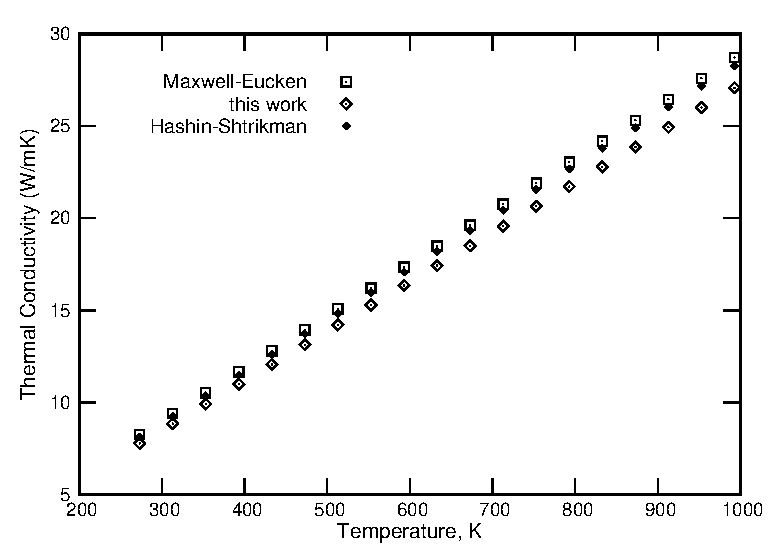
\includegraphics[width=110mm]{theory_compare_eps_rotate_bold}
	\caption[Comparison of the calculated effective thermal conductivity of \mbox{U-10Mo} with intra-granular xenon bubble (radius 1.55~nm, 10$\%$ porosity) with the Maxwell--Eucken and Hashin--Shtrikman models]{Comparison of the calculated effective thermal conductivity of \mbox{U-10Mo} with intra-granular xenon bubble (radius 1.55~nm, 10$\%$ porosity) with the Maxwell--Eucken~\cite{maxwell1881treatise} and Hashin--Shtrikman~\cite{hashin1962variational} models. In all cases, we find that the
      two theoretical models over-predict the thermal conductivity by about
      5--10~percent compared with the numerical solution.}
	\label{fig_compare}
\end{figure}

%The Hashin--Shtrikman limit agrees well with our results.
Figure~\ref{fig_compare} shows the effect of distributed gas bubbles in the intra-granular region (grain boundary bubbles were not included). Both theoretical models over-predict the conductivity by 5--10~percent, and the absolute error increases with temperature.

\subsubsection{Inter-Granular Bubbles}
Inter-granular fission gas bubbles are associated with bubbles that collect on
or near grain boundaries. Bubbles are naturally drawn to grain boundaries
because of the excess volume that accompanies grain boundaries, as well as
the decreased energy associated with void formation at grain boundaries
relative to the bulk.

To evaluate the effect of inter-granular fission gas on the overall thermal conductivity, Figure~\ref{fig_Xe_SEM}b was used as the simulation domain. As can be seen in Figure~\ref{fig_Xe_SEM}, fission gas bubbles trapped on grain boundaries do not have consistent shapes. Note that this is only a snapshot in time of the grain structure: as burnup increases, the stress in the fuel changes, more fission gas is evolved, and the grains can rotate and change shape. For simplicity, the thermal conductivity values at 1 bar were used for xenon. 
It should be noted that this only includes the effect of the bubbles gathered
at the grain boundary: effects on the conductivity associated with the grain
boundaries themselves, which will result in changes in the conductivity
because of phonon scattering effects (which are a minor contribution to thermal
conductivity in metals), as well as any effects associated with U--Mo
segregation at the grain boundary, are neglected in this model.

%Xenon's thermal conductivity was kept constant at its 1~bar value (though it is still a function of temperature).
The presence of these (intra- and inter-granular) xenon bubbles decreased the thermal conductivity by more than 25~percent, as shown in Figure~\ref{fig_eff_K_GB}. According to Miller \etal~\cite{miller2012advantages},
their sample (on which our simulations are based) went through a fission density of $3.46\times10^{21}$~fission/cm$^{3}$. At this fission density, Burkes and coworkers~\cite{burkes2015thermal} found that the experimental thermal conductivity of \mbox{U-10Mo} reduced to almost 33~percent of its unirradiated value at 473~K\@. It should
be noted that the real material has a three-dimensional grain boundary structure with varying levels of fission gas at each cross section, meaning our estimates of the thermal conductivity (which effectively assume rod-like inclusions rather than spheres) will be too low. Past
studies~\cite{bakker1997using,Schulz1981} have indicated that
conductivity in the presence of inclusions is underestimated in two-dimensional
models. This suggests that the measured conductivity (33\% of the
conductivity of the unirradiated material) may be reasonably consistent with the conductivity estimated here (\ie, 25\% of the conductivity of the unirradiated material).

\begin{figure}
	\centering
	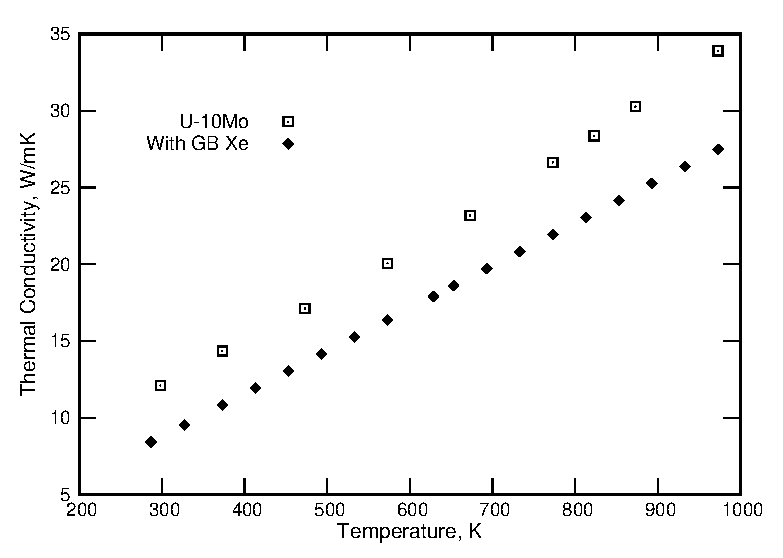
\includegraphics[width=110mm]{result_Xe_GB_eps_rot_bold}
    \caption[Comparison between the thermal conductivity of bubble-free
      \mbox{U-10Mo} with that of \mbox{U-10Mo} that has xenon bubbles
      decorating the grain boundaries according to the distribution in
      Figure~\ref{fig_Xe_SEM}]{Comparison between the thermal conductivity of bubble-free
      \mbox{U-10Mo} with that of \mbox{U-10Mo} that has xenon bubbles
      decorating the grain boundaries according to the distribution in
      Figure~\ref{fig_Xe_SEM}. A 4\% drop is observed, increasing with
      temperature.}
	\label{fig_eff_K_GB}
\end{figure}

\subsection{Effect of Xenon Pressure on the Overall Thermal Conductivity}
\label{subsec:xenonpressure}
To evaluate the impact of the pressure of the xenon bubbles on the overall thermal conductivity, we performed a study of the overall conductivity as a function of temperature for five different xenon bubble pressures given a fixed bubble distribution (Figure~\ref{gbs}b). Each pressure has a distinct thermal conductivity (Figure~\ref{fig_Xe_pressure}) as a function of temperature. In this part of the study, a constant bubble size was used (radius 1.55~nm). The results are shown in Figure~\ref{fig_press_K}. The results show little to no change of the overall thermal conductivity of the fuel due to the bubbles' pressure over the range studied. However, though xenon has a wide range of thermal conductivities at different pressures (see Figure~\ref{fig_Xe_pressure}), the effect is negligible relative to the thermal conductivity of the fuel. 

Also shown in Figure~\ref{fig_press_K} is the overall conductivity of the
system in Figure~\ref{gbs}b for bubbles filled with an 85\% xenon, 15\%
krypton mixture, with the mixture's conductivity given by
Equation~\eqref{eq:K-mixture}, using pure-component conductivities at both
1~bar and 1000~bar.  The overall conductivity is nearly identical
in all cases, indicating that the overall conductivity is not a strong
function of pressure or composition under these conditions.

\begin{figure}
	\centering
%scale=.43
	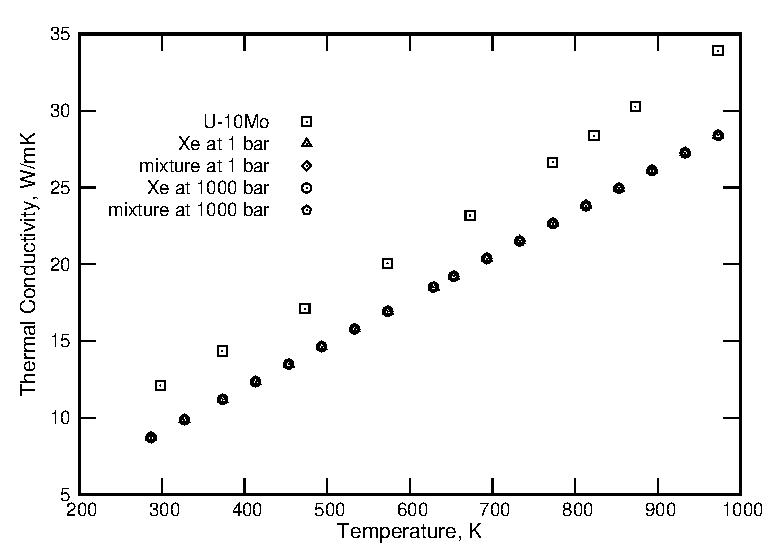
\includegraphics[width=100mm]{press_eff_k_rotate_bold}
	\caption[Overall thermal conductivity of \mbox{U-10Mo} using the thermal 
        conductivity of xenon at two extremes of pressure
        (1~bar and 1000~bar), compared to that of pure (bubble-free) \mbox{U-10Mo}]{Overall thermal conductivity of \mbox{U-10Mo} using the thermal 
        conductivity of xenon at two extremes of pressure
        (1~bar and 1000~bar), compared to that of pure (bubble-free) \mbox{U-10Mo}.
        Bubbles are distributed as in Figure~\ref{gbs}b with radii of 1.55~nm.
        {Also shown for reference is the effective thermal
        conductivity that would result from the same bubbles filled with a
        15~atom\% krypton, 85~atom\% xenon mixture (representative of fission
        gas) at both 1~bar and 1000~bar.}}
	\label{fig_press_K}
\end{figure}
%Based on our results, xenon bubbles reduces the thermal conductivity more than 25$\%$. The experimental thermal conductivity reduces much more. This is due to several factors. Fission bubbles have a wide range of sizes and shapes. Also thermal conductivity of U-Mo system is sensitive to the Mo concentration. It decreases with the increase of molybdenum concentration~\cite{kaufmann1962nuclear, burkes2015thermal}. Because molybdenum is a fission product, it further enhances. There is a diffusion barrier between the Aluminum cladding and fuel, which is usually Zr. These two layers create the contact resistance, that would affect the heat flow.

\subsection{Effect of Bubble Arrangement on Thermal Conductivity}
\label{subsec:area}
We performed a series of simulations to determine whether bubble distribution has a significant influence on the overall thermal conductivity. Two cases were considered. In the first case, we used same number (16) of bubbles of the same diameter (1 nm) and organized them into five different arrangements. The arrangements are arbitrary, but each has the same area fraction of bubbles (xenon gas). In the first arrangement (Figure~\ref{fig:five_figures}a), the bubbles are dispersed uniformly throughout the domain. In Figure~\ref{fig:five_figures}b, the bubbles are arranged in a denser pattern with bubble-free portions near the high-temperature side. In Figure~\ref{fig:five_figures}c, the bubbles are arranged in one corner. In Figure~\ref{fig:five_figures}d, the bubbles are tightly clustered near the center of the domain, creating significant bubble-free regions at the top and bottom. The overall thermal conductivities for these arrangements are presented in Figure~\ref{fig:five_results}.
In these simulations, heat is flowing from left to right, whereas the top and bottom boundaries are insulating (adiabatic).

Based on the results from Figure~\ref{fig:five_figures}, arrangement (d) shows a minor deviation, particularly at high temperatures, compared to the other arrangements. The other four bubble arrangements do not produce significantly different thermal conductivities. The reason for the deviation for case~(d) is the relatively wide ``heat channel'' in the direction of the heat flow, which is absent in the other arrangements. The highest thermal conductivity difference between Figure~\ref{fig:five_figures}d and the other arrangements is approximately 0.93~W/m$\cdot$K, which is also a function of the open channel's area.

\begin{figure}
	\centering
	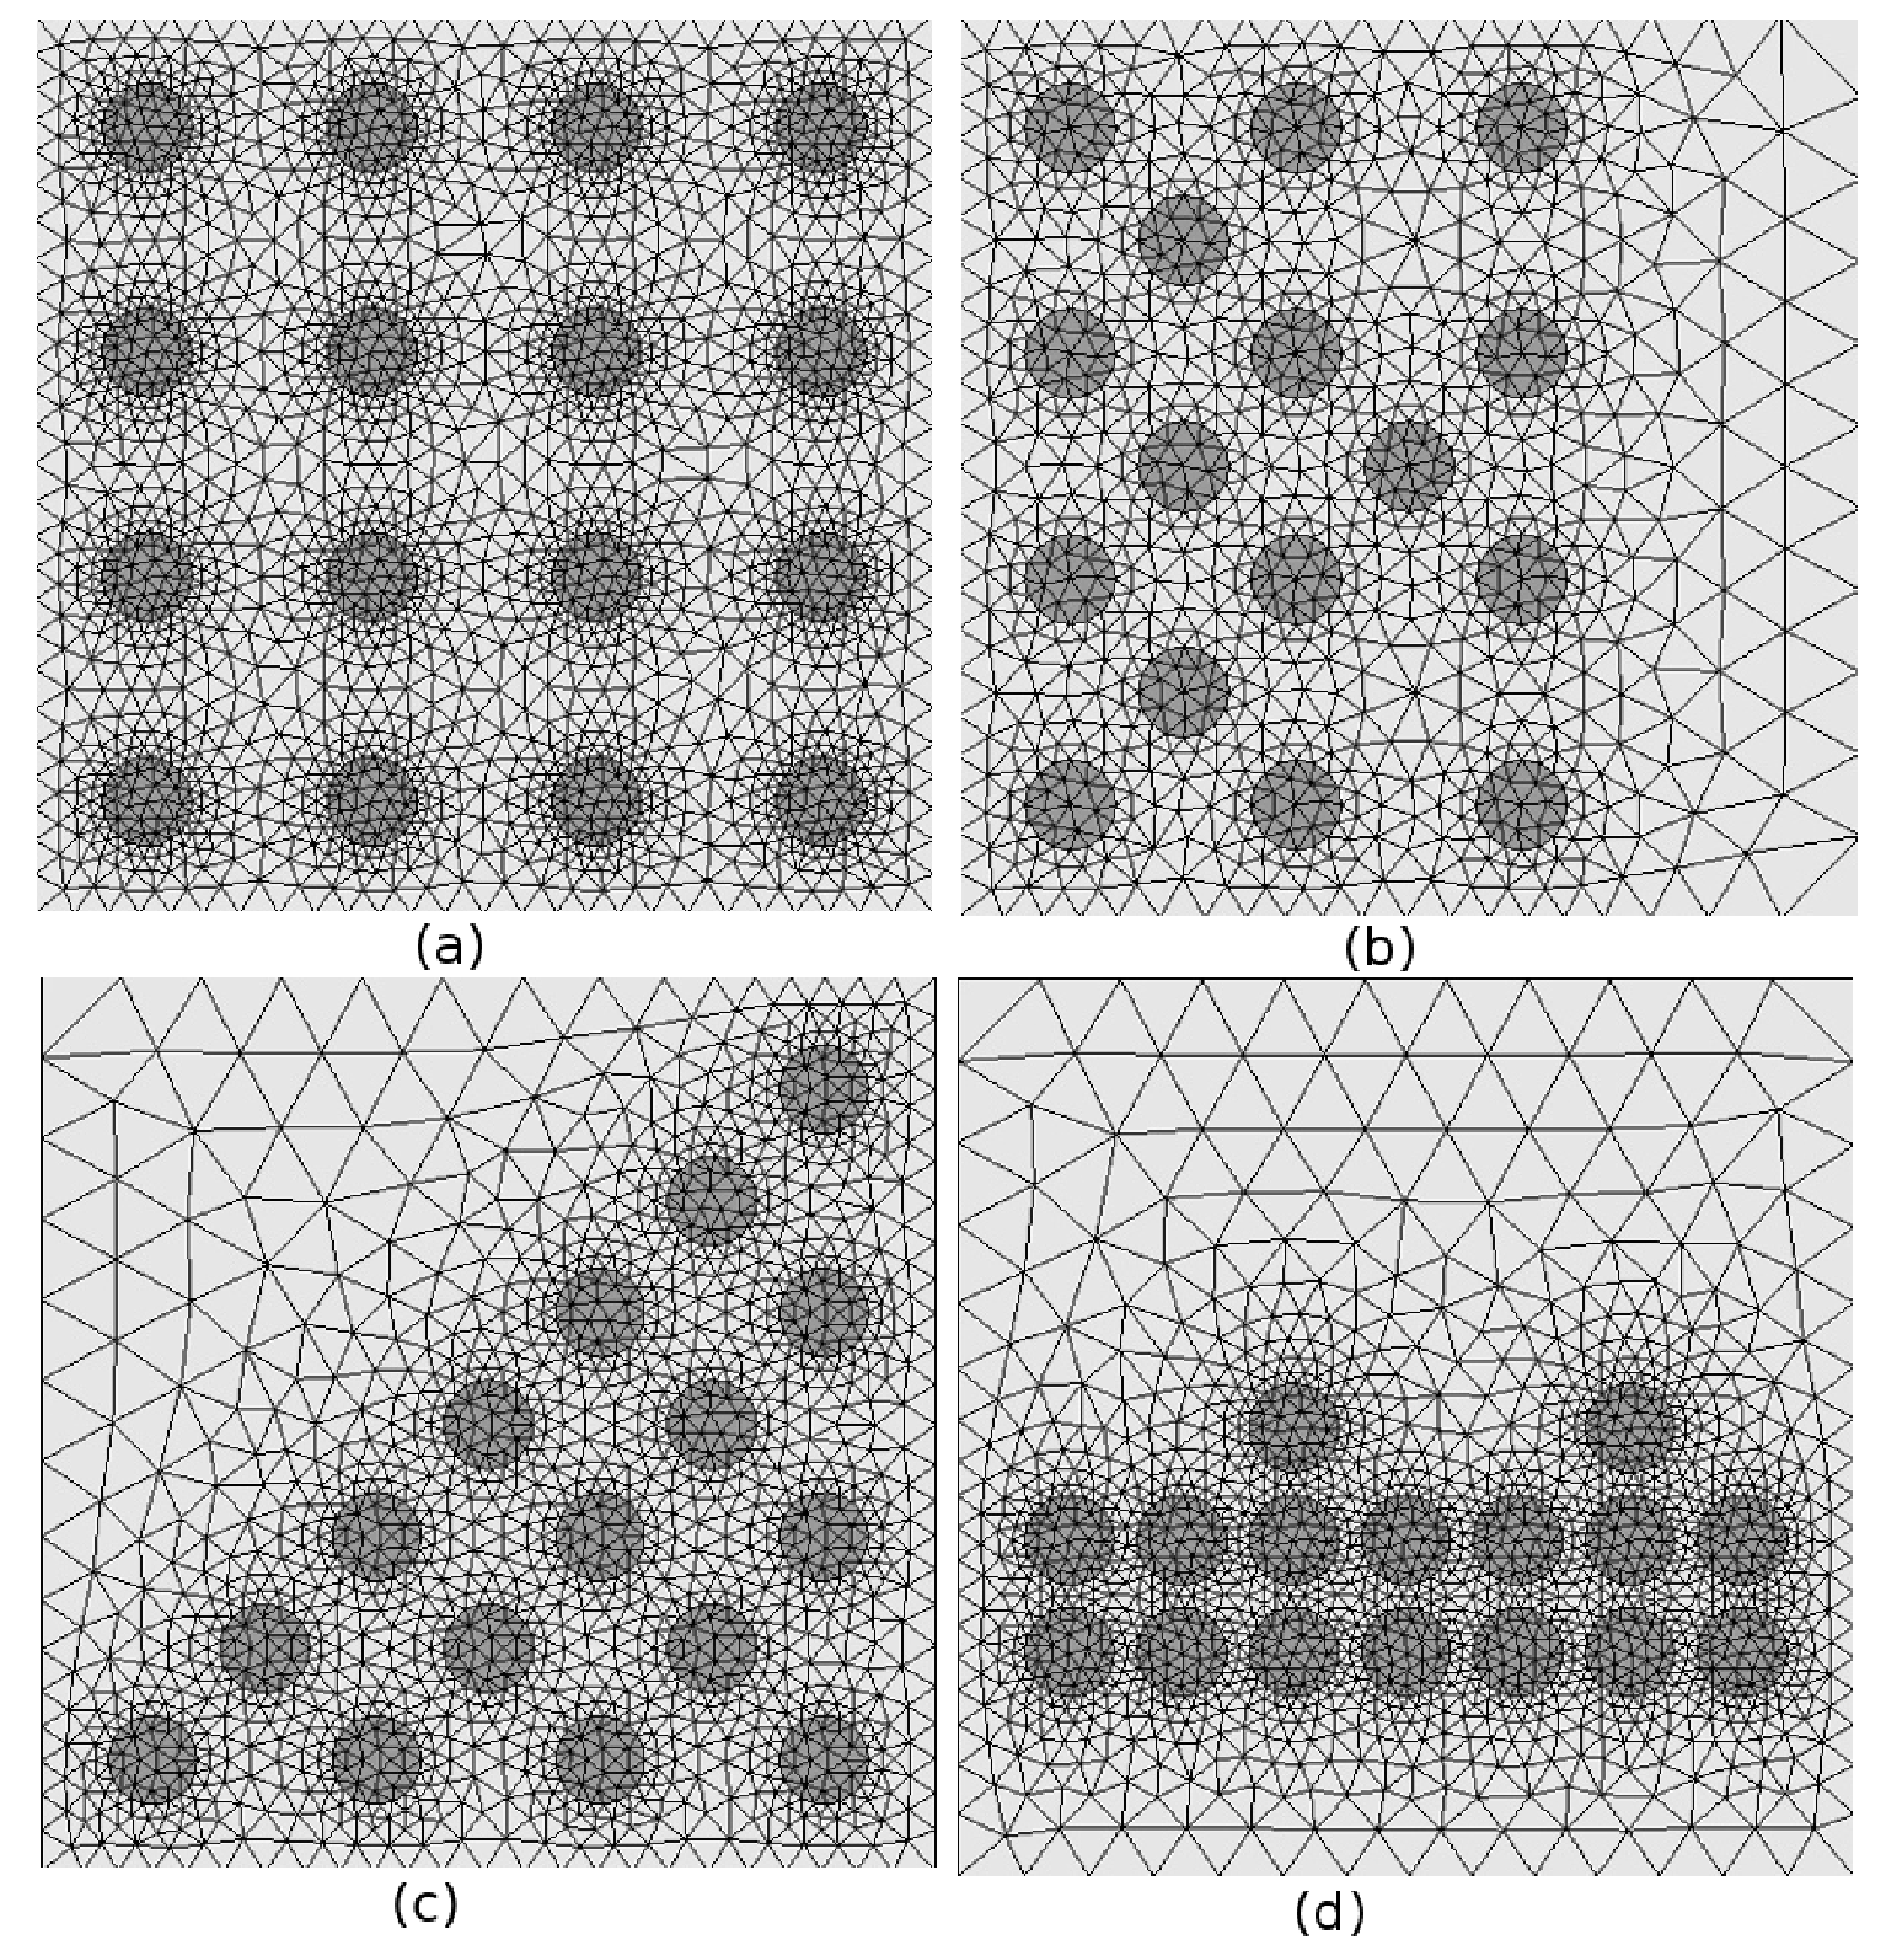
\includegraphics[width=110mm]{2x2_abcd_gray}
    \caption[Different bubble arrangements in which the area of each bubble and
      the number of bubbles are the same]{Different bubble arrangements in which the area of each bubble and
      the number of bubbles are the same. Heat flows from left to right in
      these simulations; only arrangement (d), with its uninterrupted ``heat
      channel'' in the top half of the domain, shows significantly different
      conductivity.}
	\label{fig:five_figures} 
\end{figure}

\begin{figure}
	\centering
	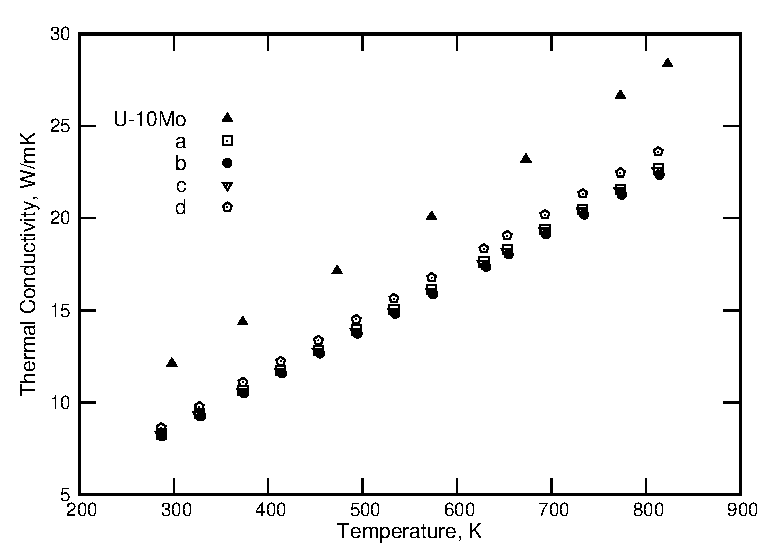
\includegraphics[width=110mm]{result_area_compare_eps_bold_rotate}
    \caption[Comparison of the calculated thermal conductivity of different
        bubble arrangements (constant bubble area and diameter corresponding to Fig.~\ref{fig:five_figures}). ]{Comparison of the calculated thermal conductivity of different
        bubble arrangements (constant bubble area and diameter corresponding to Fig.~\ref{fig:five_figures}). Only
        arrangement (d), with its properly-oriented ``heat channel,'' shows significant
        differences from the others, and such differences are relatively
        insignificant compared to the bubble-free conductivity.}
	\label{fig:five_results}
\end{figure}

In the second case, different bubble sizes were used with constant total area. As the first case shows, bubble arrangement has minimal impact on the overall heat transfer unless it produces a significant heat transfer channel in direction of the heat flow. In this step, we kept the total area covered by the bubbles the same, but with different sizes of bubbles. To keep the area same while decreasing the bubble diameter, the number of bubbles increases. Figure~\ref{fig:area_same_four} shows the four different arrangements with different bubble sizes. None of the arrangements creates a heat transfer channel in the direction of heat flow. The results are shown in Figure~\ref{fig:four_results}. The results show no significant change in the overall thermal conductivity. We conclude that the bubble arrangement has little impact unless it produces a significant bubble-free heat transfer channel. 

 
\begin{figure}
	\centering
	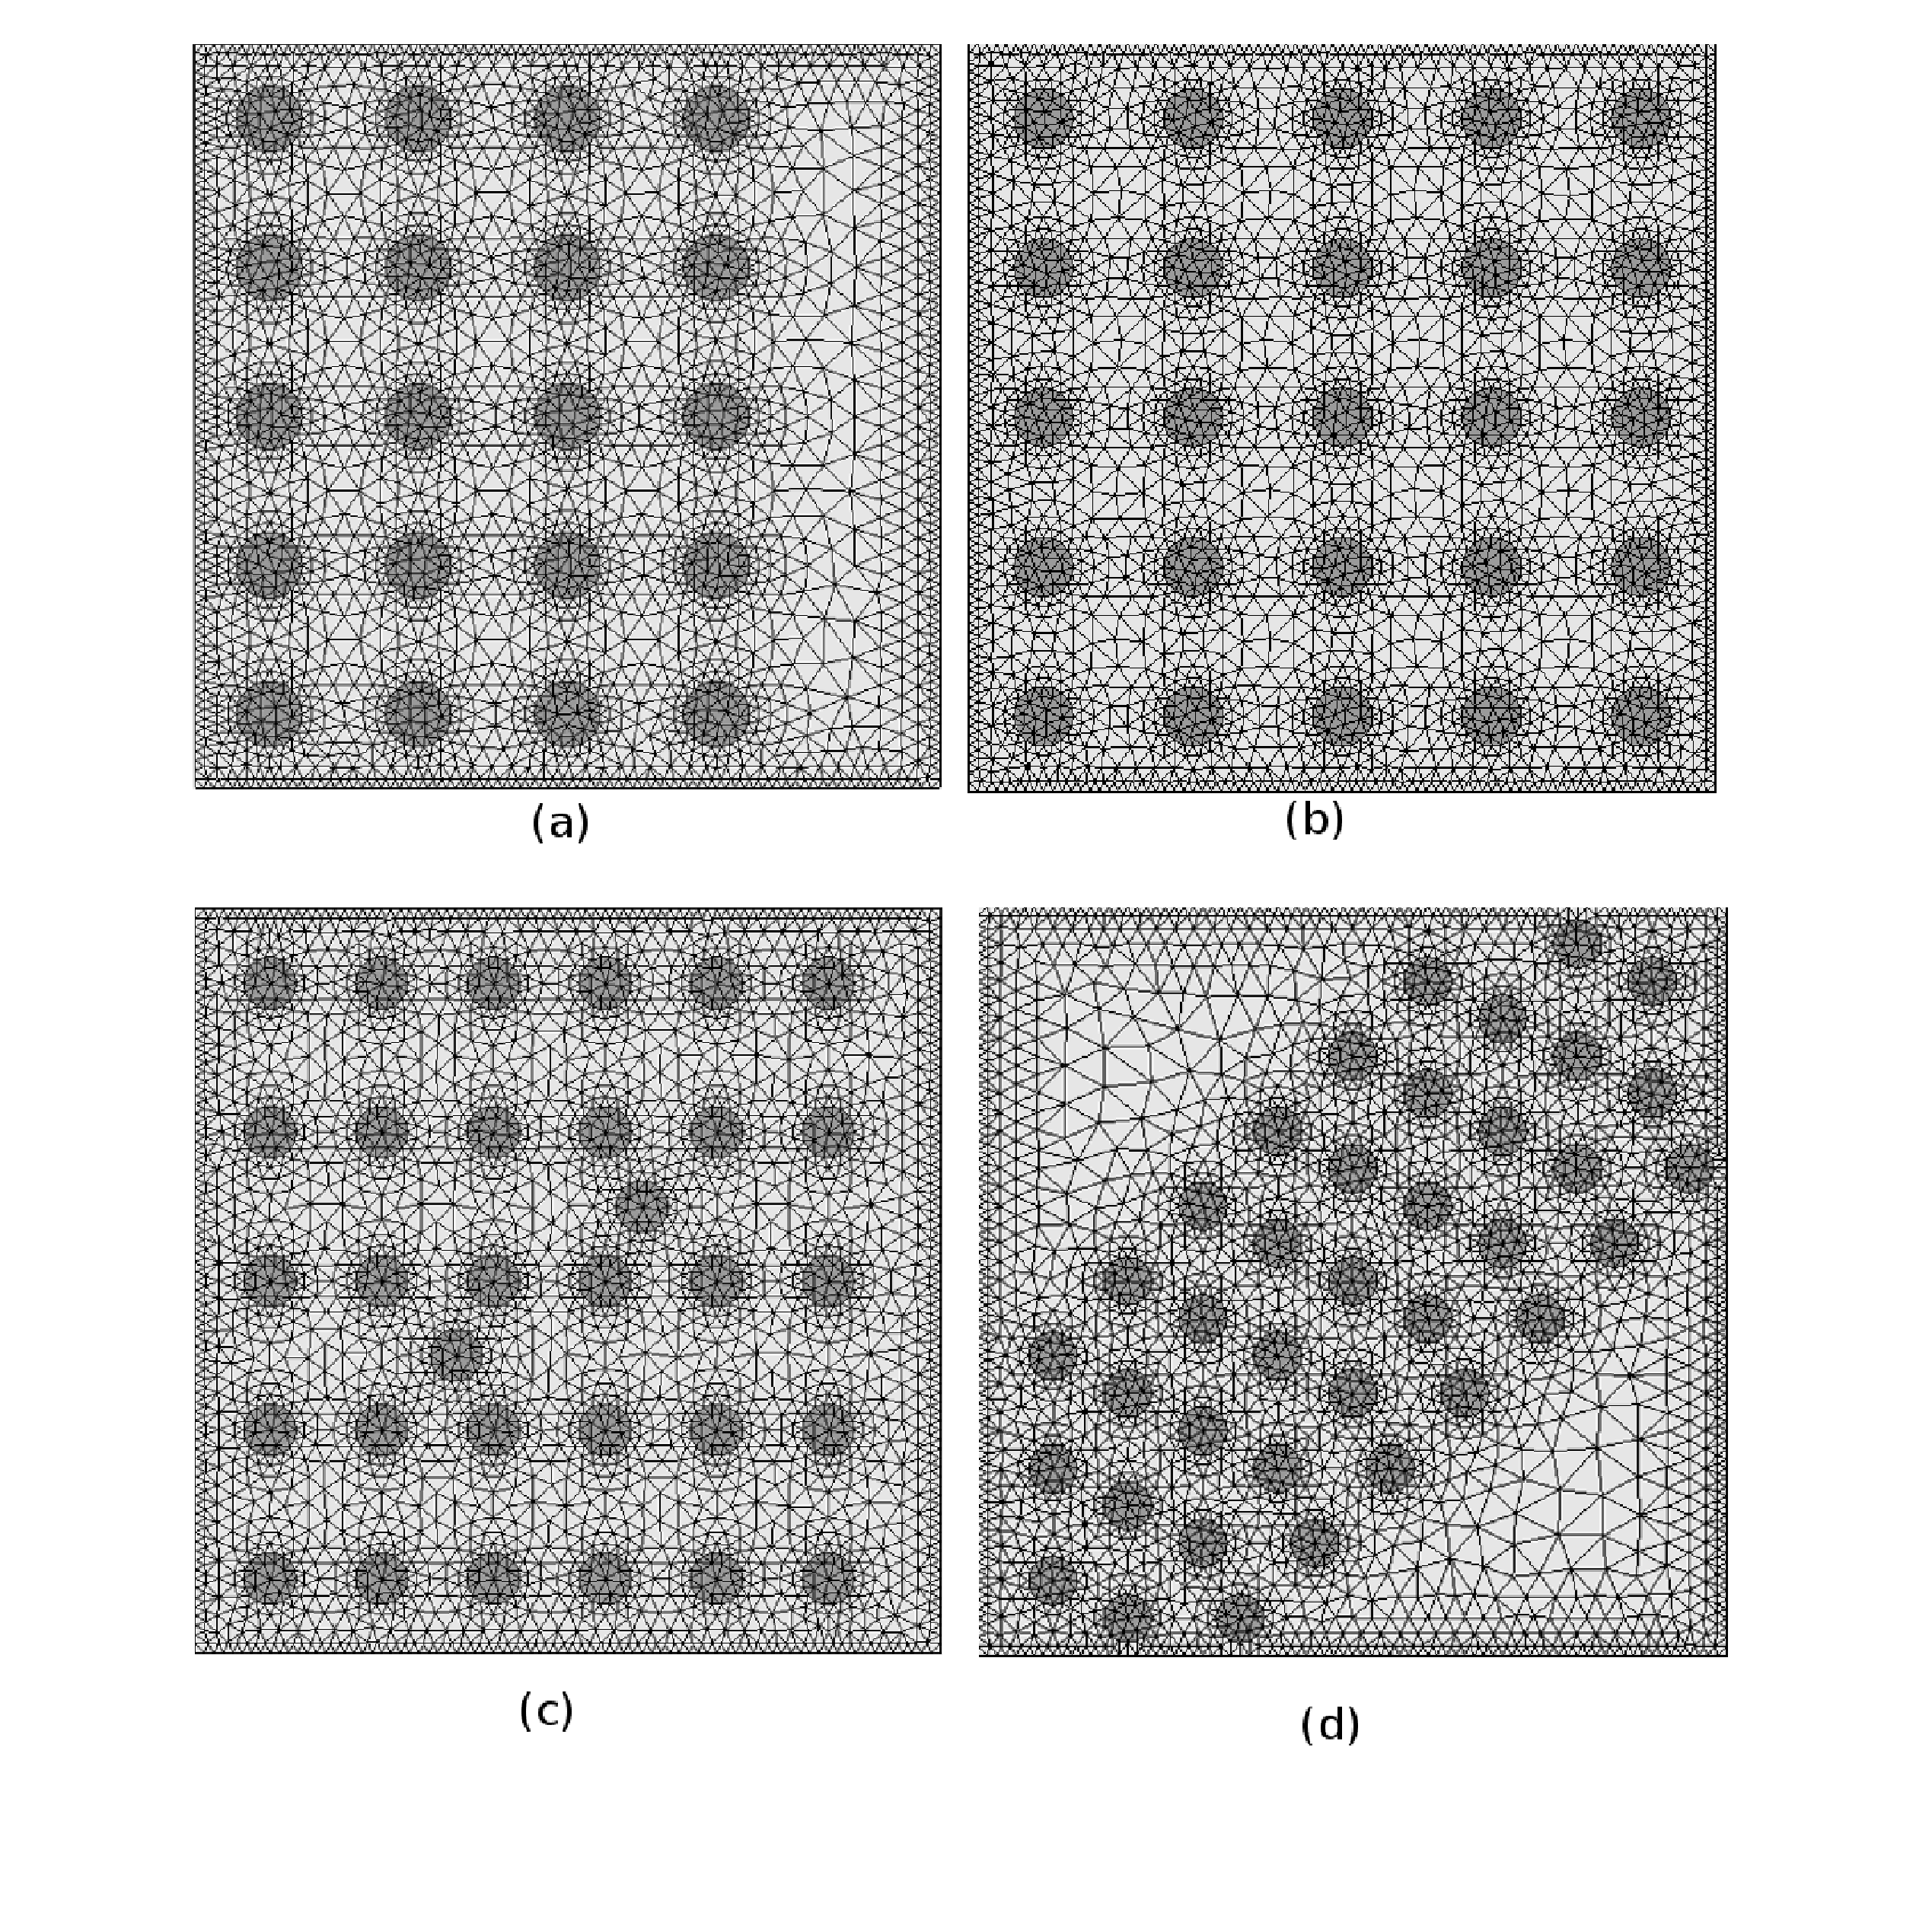
\includegraphics[width=110mm]{same_area_four_figure_gray}
    \caption{Different bubble arrangements where the area is the same but the
      bubbles have different diameters. (a)~20 bubbles, (b)~25 bubbles,
      (c)~32 bubbles, (d)~38 bubbles.}
	\label{fig:area_same_four}
\end{figure}
\begin{figure}
	\centering
	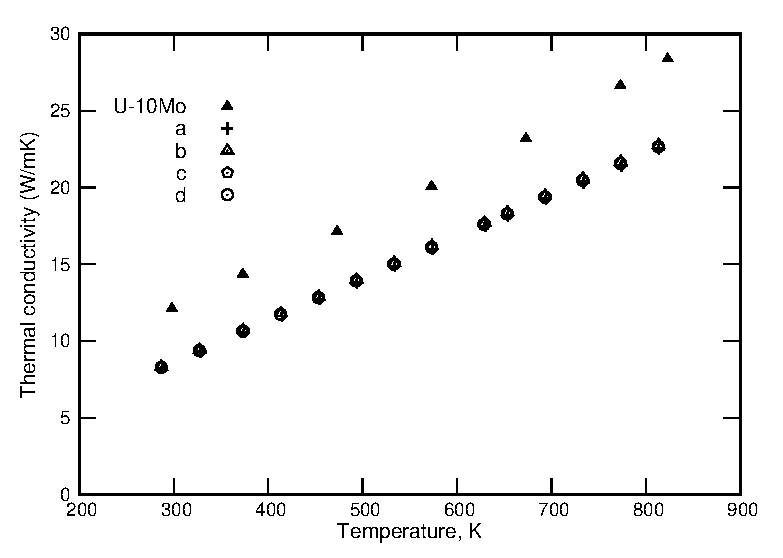
\includegraphics[width=110mm]{area_same_result}
	\caption[Comparison of thermal conductivity between different bubble 
      diameters at constant total bubble area with bubble-free U-10Mo. Bubble
      arrangements are shown in Figure~\ref{fig:area_same_four}]{Comparison of thermal conductivity between different bubble 
      diameters at constant total bubble area with bubble-free U-10Mo. Bubble
      arrangements are shown in Figure~\ref{fig:area_same_four}.
      Bubble diameters are (a) 0.894 nm (b) 0.8 nm (c) 0.707 nm and (d) 0.6488 nm;
      the bubble area fraction is 12.6$\%$~percent.}
	\label{fig:four_results}
\end{figure}

%this is the new addition on the discussion
In our calculation, grain boundary xenon gas bubbles had very minimal impact on the overall heat transfer. That is because our sample has very low grain boundary fission gas areal density, less than 2$\%$ of the total area. Grain boundary fission gas bubble size increases with an increase in burnup~\cite{kim2011fission}.
With an increase in fission density, more fission gas usually diffuses to the grain boundary area and recrystallization~\cite{kim2013recrystallization} subdivides the grains to accommodate the fission gas near the grain boundaries.
This also increases the grain boundary fission gas density. Our results were also compared with porosity correction models, specifically those of Bauer~\cite{bauer1995pile} and Peddicord~\cite{peddicord1978porosity}. Bauer's model ($\lambda=\lambda_0 e^{-2.14\nu}$, where $\lambda_0$ is the thermal conductivity of the 100\% dense material and $\nu$ is the porosity) over-predicts the porosity correction factor for thermal conductivity. Peddicord's model ($\lambda=\lambda_0(1-\nu)^{2.58}$) agrees better with the effective thermal conductivity from our simulations. All these empirical models are applicable to intragranular gas bubbles with uniform distribution and negligible fission gas thermal conductivity.
In our calculation, all the thermal conductivities are measured from two-dimensional finite element models, but two-dimensional thermal conductivity usually represents the lower limit of the three-dimensional thermal conductivity~\cite{bakker1995determination}. Accurate estimation of this limit is very important. 

\section{\label{sec:conclusion}Conclusions}
Estimating the thermal conductivity of nuclear fuel is an important part of understanding fuel behavior in nuclear reactors. In our work, xenon gas was used to represent fission gas bubbles in \mbox{U-10Mo} monolithic fuels. The impact of distributed xenon bubbles on the overall thermal conductivity of \mbox{U-10Mo} is significant, resulting in a 25--35~percent drop in conductivity for the bubble volume fractions studied, largely independent of bubble arrangement. Both intra- and inter-granular gas bubble structures were used. For intra-granular bubbles, a gas bubble superlattice structure was used. The results indicate that the Maxwell--Eucken and Hashin--Shtrikman models overestimate thermal conductivities by at least 5\% for the bubble volume fractions studied.

The pressure dependence of xenon's thermal conductivity was also studied to estimate the impact of bubble pressure on the overall thermal conductivity of \mbox{U-10Mo}. Our results indicate that bubble pressure is not a significant factor for the bubble densities studied---the overall thermal conductivity remains largely unchanged between 1~bar and 1000~bar.
We also find that there is little difference between pure xenon bubbles and
85\% xenon--15\% krypton bubbles from the perspective of overall thermal
conductivity in bubble-laden \mbox{U-10Mo}.

We find that both intra- and inter-granular xenon bubbles reduce the overall thermal conductivity by more than 25~percent. Different bubble arrangements have very little impact on the overall heat flow, unless the arrangement leads to a significant bubble-free channel through which heat can be conducted without interference from nearby bubbles. Bubble size is also not a significant factor, as different bubble sizes at the same bubble areal density produce a U-10Mo slabs with identical overall conductivity.

{We did not consider the effects of solid
fission products and their influence on the overall thermal conductivity. We
believe that this issue needs a complete and thorough investigation, because the
chemical state and the distribution of the solid fission products of U--Mo may
make important contributions to the overall conductivity.}
Future work should also study, quantitatively, the contact resistance between
the cladding and fuel, as well as the evolution of grain boundaries with time
and the influence of local molybdenum concentration on thermal conductivity.




%\bibliographystyle{iopart-num}
\bibliographystyle{apsrev4-2}
\bibliography{abbreviated,final}
%\bibliography{abbreviated,xnthrm}
